\documentclass[paper=a4,12pt,DIV=11,twoside=false]{scrartcl}
%\usepackage[dvips]{graphics}
\usepackage[english]{babel}
\usepackage{graphicx}
\usepackage{amsmath}
\usepackage{natbib}
%\setlength{\bibsep}{0pt plus 0.3ex} % reduce spacing in bibliography
\usepackage{multibib} % appendix bib
\newcites{sec}{Other Sources} % appendix bib
\setcitestyle{notesep={; },round,aysep={},yysep={;}}
%\usepackage{cite}
\usepackage{multirow}
\usepackage{pgf}
\usepackage{lscape}
\usepackage{setspace}
\usepackage{subfigure}
\usepackage{rotating}
\usepackage{comment}
\usepackage{graphicx}
\usepackage{threeparttable}
\usepackage{color}
\usepackage{colortbl}
\usepackage{appendix}
\usepackage{changes}
\usepackage[pdftex,colorlinks=true,linkcolor=black, citecolor=black, urlcolor=black]{hyperref}
\usepackage{standalone} % ignore the preamble in the appendix
\usepackage{longtable} % multi-page tables
%\usepackage{subcaption}
\usepackage{csquotes}
\colorlet{Changes@Color}{red}
\newcommand{\colorr}{ \color{red} }
\newcommand{\colorb}{ \color{blue} }
\newcommand{\colorg}{ \color{green} }
\newcommand{\colory}{ \color{yellow} }
\newcommand{\colorm}{ \color{magenta} }
\newcommand{\colorc}{ \color{cyan} }
\newcommand{\possessivecite}[1]{\citeauthor{#1}'s (\citeyear{#1})}
\renewcommand\appendixpagename{Appendices -- Not For Publication}  % AER style appendix page as against "Appendices"
% from appendix preamble

%\setlength{\oddsidemargin}{.05 in}% {.5 in}
%\setlength{\textwidth}{6.25 in}%6{5.5 in}5.9
%\setlength{\textheight}{680pt}
%\setlength{\topmargin}{-50pt} %-40pt NO DEFAULT-15 25
%\setlength{\footskip}{25pt} %NO DEFAULT 40pt

%\addtolength{\topmargin}{-0.375in}
%\addtolength{\oddsidemargin}{-0.35in}
%\addtolength{\evensidemargin}{-0.35in}
%\addtolength{\textheight}{0.5in}
%\addtolength{\textwidth}{0.5in}
%\addtolength{\parskip}{0.05em}
%\setlength{\parindent}{0.6cm}
%\parskip = .12 in
\KOMAoptions{parskip=half}

\renewcommand{\baselinestretch}{1.5}
\newcommand{\vsp}{\vspace{\baselineskip}}
\newcommand{\be}{\begin{equation}}
\newcommand{\ee}{\end{equation}}
\newcommand{\gr}[1]{\ensuremath  {\frac{\dot {#1}}{#1}}}
\newcommand\T{\rule{0pt}{2.6ex}}
\newcommand\B{\rule[-1.2ex]{0pt}{0pt}}
\newcolumntype{L}[1]{>{\raggedright\let\newline\\\arraybackslash\hspace{0pt}}m{#1}}
\newcolumntype{P}[1]{>{\raggedright\arraybackslash}p{#1}}
\newcolumntype{C}[1]{>{\centering\let\newline\\\arraybackslash\hspace{0pt}}m{#1}}
\newcolumntype{Q}[1]{>{\centering\let\newline\\\arraybackslash\hspace{0pt}}m{#1}}  

%\pretolerance10000\tolerance10000\hbadness10000 \textwidth
%6.5in\textheight 9.25in\oddsidemargin 0in\evensidemargin 0in
%\topmargin      -0.2in\headheight 0in\headsep        0in




\begin{document}



\title{When Mistrusting Experts Pays Off}
\subtitle{Persuasive Signalling when Transparency is Costly}
\author{
Selina Hofstetter
}	

\maketitle

\begin{abstract} 
\singlespacing

\noindent In situations of information asymmetry, how do two independent agents communicate when they share the same objective, but transparency is costly due to negative externalities or exponentially increasing effort to explain communicated content? This paper presents a formal model where the sender of a signal chooses the variance in the signal's probability distribution dependent on the receiver's prior about the state of the world and his belief about the sender's transparency. Results show that having not too trusting receivers can increase average precision levels in the signal - an outcome resembling an accountability effect. Further, the model shows that variation in priors among the receivers also increases signal precision. At last, negative externalities that the signal induces on third parties constrain the sender's transparency. A policy implication that follows from this is that exclusive communication channels between experts and legislators can be welfare-enhancing. The model complements empirical results on the communication between the US Federal Open Market Committee and the US Congress in the period 1993-2010 \citep{GL2017}.
\end{abstract}

\newpage
\tableofcontents
%\vspace{8em}
\clearpage
\listoffigures

\newpage

\onehalfspacing


% ============================================== %
% SECTION == PAPER =========================== %
% ============================================== %

\section{Introduction}

\begin{displayquote}
\begin{flushright}
\textit{"Trust is good, but control is better."}\\
\textit{\textbf{Vladimir Lenin}}
\end{flushright}
\end{displayquote}

\noindent Even though the political economy literature mainly focuses on strategic communication between two parties that have differing objectives (e.g. a biased committee providing policy information to a legislative body), a large part of information exchange happens between individuals sharing the same ideal outcome. In those situations, the sender (she) would like to pass on an unbiased message to the receiver (he). From cheap talk games we learn that she succeeds when signalling is cost-free.\footnote{That is when both sender and receiver have no bias and signalling is free (hence "cheap talk"), then the sender can send a fully revealing signal to the receiver. Regular cheap talk games however consider situations in which the sender has a bias.} This paper looks at communication outcomes when the sender bears a cost that increases in her signal's precision. Hence, she faces costly transparency. We can think of two intuitions behind such cost: (1) The sender has to exert effort to explain her message's content to the receiver. Communication may fail, because the cost of effort is increasing faster than the benefit from the receiver's comprehension. (2) The signal's precision induces negative externalities when a third party also listens and reacts to the message content in a way that works against the sender's objective. Communication may fail, as the sender's incentive to be precise is too constrained by her fear of causing externalities. An example for (1): In school or at work, providing insight to more complex information allows a better understanding of an issue, but the required effort to explain is often an exponential function of the amount or depth of the transmitted information. If someone reveals more information (i.e. being more transparent) without explaining it, she risks that the information is misunderstood and induces the wrong action. So it may be better to reveal less, but explain it at relatively low cost of effort. \citet{DT2005} show how successful communication depends on the effort that both sender and receiver put into understanding each other. When the receiver's ex-ante expected payoff from implementing an action $a_R$ is positive, the sender will put no effort into the information transmission about $a_R$ (which she wants the receiver to implement). Thus, if transparency (i.e. precision in the signal sent about $a_R$) would require effort, the sender would exert none in equilibrium, while the receiver would still choose action $a_R$ due to his prior belief that it will bring him on average a positive payoff. This will however not happen in this paper's model, as what here also matters is the receiver's belief about the sender's transparency.\footnote{Hence, if the sender would send a completely unprecise signal, while the receiver believed him to be quite transparent, both would be at risk of the receiver updating his prior and consequently choosing the wrong action, despite his prior being biased towards the true state of the world.} An example for (2): We can think of the letter exchange between Queen Victora and Prince Albert when a third party would always read their messages too such that speaking entirely open to each other imposed the risk of offending the third party, even though both would have preferred straightforward communication. Or in the case of the Federal Open Market Comittee's (FOMC) communication with the US Congress, the third party hearing and reacting to the FOMC's information are the financial markets. Each signal that the FOMC sends to US Congress in the form of publishing FOMC minutes also reaches them and may induce disadventageous market behaviour. For example, if the FOMC would like the US Congress to increase government expenditure as an ideal complement to the Fed's expansive monetary policy, the financial markets will pick up on a clear signal implying a bad state of the economy. As a consequence, banks may be more reluctant to issue credit, which works against the FOMC's intention to revive the economy. Thus, there are obvious incentive constraints to the FOMC's communication transparency, even though it would like to openly tell Congress that the economy needs its policy support.

In the following model, I consider both possible forms of cost to precise signalling through an exponential cost function that depends on the signal's distribution variance. First, the results I derive show that variance decreases in equilibrium when the sender needs to use more persuasive evidence to convince the receiver. That is when the receiver has a low prior while the state of the world requires high action, or vice versa. Second, equilibrium precision levels increase even more when the receiver further believes that the sender's transparency is low. Which means that the signal's distribution variance decreases, the higher the receiver believes it to be. This identifies a form of accountability effect, as the receiver's mistrust incentivises the sender to become more trustworthy. However, this only occurs in combination with the need for persuasion (see first result). Whenever the receiver already holds the correct prior, then the sender has no incentive for high precision in his signal. At last, I compare these results to recent empirical evidence on variation in the FOMC's communication transparency with US Congress (\citet{GL2017}), where the percentage of overlapping wording in the published FOMC meeting minutes and the 5 years later released transcripts serve as transparency indicator. My model's results suggest an extension to the current empirical research design, which would include a binary variable for a Republican majority in either Senate or House. They further suggest a control variable for shifts in party priors over time, which may be able to test the hypothesis that the FOMC becomes more transparent when the need for persuasive evidence increases. The paper is structured into a review of the current literature on costly signalling and persuasion, the description of the model and its equilibrium in pure strategies, the derived comparative statics and finally the conclusion with a research outlook. The Appendix provides the relevant proofs.

\section{Literature}

\noindent Most models on political communication exploit differing objectives in a principal-agent relationship or between a biased expert and a decision-making audience. Signalling in these models is usually cost-free, or they introduce a cost to allow for a separating equilibrium with truthful information transmission. The most prominent model on strategic communication is the one by \citet{CS1982}, which built the basis for a continuously growing literature on cheap talk. Bayesian persuasion models such as the one by \citet{KG2011} eliminate the sender's ability to pass on biased information (e.g. because he is legally bound to tell the truth with otherwise severe punishment), but still assume differing objectives between sender and receiver. The sender has a first-mover advantage, as she can acquire only as much information as is optimal for her, given that the receiver best responds by listening to the transmitted information, updating his prior. In equilibrium, the receiver (a judge) convicts a higher percentage of people than are actually guilty in the population. Which is an outcome favourable to the sender (a prosecutor), but not the receiver. \citet{DT2005}, on the other hand, look at communication that has a continuously increasing cost in persuasion. That is, both sender and receiver need to exert effort in order to explain or understand the signal sent, which allows the receiver to update his prior and make a decision on whether to take the sender's recommended action $a_R$ or not. 

\noindent The model I present in this paper differs from the existing literature in two main aspects. First, both sender and receiver have an identical objective, i.e. that the state of the world $\theta$ should exactly match the receiver's implemented action $a_R$. Second, the sender can choose the precision degree $\sigma^2$ of the distribution from which the receiver draws a signal. Hence, the sender has control over the spread of possible messages but not over the exact message arriving at the receiver, unless he chooses $\sigma^2=0$. This can be interpreted as having control over the level of transparency in communication. Full transparency requires zero variance in the signal's distribution, which would ensure that the receiver gets and fully understands the exact information that the sender passes on. I assume that only the sender bears an exponential cost of transparency. Third, the receiver holds not only a belief about the state of the world, but also about the level of transparency with which the sender communicates. I state this belief as $\hat{\sigma}^2$. It is the prior beliefs on both $\theta$ and $\sigma^2$, which generate interesting results for the comparative statics analysis that follows later in the paper.

\section{The Model}

\noindent In the following, I provide the set-up, timing and assumptions of my model before I derive the equilibrium occurring under the given conditions. I explain the essential model assumptions in detail and introduce an extension to the model at the end, which allows for an interesting empirical interpretation.

\subsection{Set-up and Timing:}

\begin{itemize}
\item Two agents: Sender $S$ (she) and receiver $R$ (he)
\item $S$ has access to exclusive information, i.e. she receives a private signal at the beginning of the game, which fully informs her about the state of the world $\theta \in \{0,1\}$. She wants $R$ to choose the right action $a_R$ that matches the state of the world, but she also cares about the cost of transparency. Her objective function takes the following form: 

\begin{equation}
U_S = -(a_R - \theta)^2 - c(\sigma^2)
\end{equation}

\item She chooses a level of transparency $\sigma^2$ to send a signal $s(\theta)\sim(\theta, \sigma^2)$ about the state of the world to $R$. So the higher the variance in the signal's distribution, the lower the transparency the sender chooses to communicate what $\theta$ is and vice versa
\item Transparency comes at an exponential cost $c(\sigma^2) = e^{(-\sigma^2 + b)}$ for the sender, where $b$ is a constant determining the baseline cost for full transparency, i.e. when $\sigma^2=0$. Costs decrease in $\sigma^2$, i.e. $\dfrac{dc(\sigma^2)}{d\sigma^2} < 0$ and $\lim_{\sigma^2 \to +\infty} c(\sigma^2) = 0$. Thus, higher levels of transparency cost exponentially more than lower levels
\item As in the case of Bayesian persuasion, $S$ cannot lie about the state of the world, which means she cannot upward- or downward-bias the mean in the signal's distribution (i.e. she cannot choose $s(\theta)\sim(\theta+b, \sigma^2)$ or $s(\theta)\sim(\theta-b, \sigma^2)$). She can only determine the variance in the distribution. So whenever $\sigma^2=0$, the signal would be fully revealing $\theta$ at cost $c(0)= e^{(b)}>0$
\item $R$ holds a prior probabilistic belief $\pi(\theta=0)\in \big[0,1\big]$ about the state of the world and an \textit{exogenous}, non-probabilistic one about the level of transparency in $S$'s communication $\hat{\sigma}^2\in \big[0,+\infty\big]$. Non-probabilistic meaning that he is convinced of a certain degree in the signal's distribution $\sigma^2 = \hat{\sigma}^2$
\item Upon receiving the signal, $R$ updates his prior $\pi(\theta=0)$ about the state of the world using Bayes rule. He decides based on his posterior $\pi(\theta=1|s, \hat{\sigma}^2)$ what action $a_R \in \{0,1\}$ to take. He wants to choose the right action that matches the state of the world. His objective function is therefore: 

\begin{equation}
U_R = -(a_R - \theta)^2
\end{equation}
\end{itemize}

\subsection{The Equilibrium:}

\noindent We look for a Perfect Bayesian Equilibrium (PBE) in pure strategies. Given that $S$'s signalling is unbiased, $R$'s best response is to choose $a_R=1$ whenever $\pi(\theta=1|s, \hat{\sigma}^2) > 0.5$. And whenever $\pi(\theta=1|s, \hat{\sigma}^2) < 0.5$, he best responds by choosing $a_R=0$. When $\pi(\theta=1|s, \hat{\sigma}^2) = 0.5$, he tosses a coin. His best response function therefore takes on only binary values: $a_{R}^{*}(s,\hat{\sigma}^2)\in \{0,1\}$ for all possible values of $s$, $\sigma^2$ and $\hat{\sigma}^2$. In order to show that listening to the signal is always the weakly dominant strategy for $R$ we can consider the case where $R$ believes $S$ to be completely intransparent, i.e. if $\hat{\sigma}^2 \to +\infty$. He is then indifferent between listening to the signal to update his prior or just ignoring it, as the signal provides essentially no new information to him. Thus, his Bayesian update simply returns his prior belief about $\theta$.\footnote{Because $\pi(s \leq s'|\theta=1, \hat{\sigma}^2 \to +\infty) = \pi(s \geq s'|\theta=0, \hat{\sigma}^2 \to +\infty)=\pi(s \leq s'|\hat{\sigma}^2 \to +\infty)$ \\ \\s.t.  $\pi(\theta=1|s, \hat{\sigma}^2 \to +\infty) = \dfrac{\pi(s \leq s'|\hat{\sigma}^2 \to +\infty)\pi(\theta=1)}{\pi(s \leq s'|\hat{\sigma}^2 \to +\infty)(\pi(\theta=1)+\pi(\theta=0))}= \pi(\theta=1)$, where $s'$ is the signal received here.}

\noindent \textbf{An Example:} A receiver with prior beliefs $\pi(\theta = 0)=0.6$ and $\hat{\sigma}^2 = 1$ receives a signal $s=0.3$. He updates his belief with Bayes rule and concludes that he should choose action $a_{R}=0$:

\begin{center}
$\pi(\theta = 0|s = 0.3,\hat{\sigma}^2=1)$ 
\end{center}

\begin{center}
$= \dfrac{\pi(s \geq 0.3 | \theta = 0,\hat{\sigma}^2=1)\pi(\theta = 0)}{\pi(s \geq 0.3 | \theta = 0,\hat{\sigma}^2=1)\pi(\theta = 0) + \pi(s \leq 0.3 | \theta = 1,\hat{\sigma}^2=1)\pi(\theta = 1)}$
\end{center}

\begin{center}
$=\dfrac{(0.3821)(0.6)}{(0.3821)(0.6)+(0.2420)(0.4)}\cong 0.7 > 0.5 \Rightarrow a_{R}=0$
\end{center}

\noindent As $s$ follows a continuous normal distribution, $R$ cannot learn the exact probability of $s=0.3$, but he can derive its p-value, i.e. the probability of receiving a signal $s \geq 0.3$ if the true state of the world were zero and the probability of receiving  $s \leq 0.3$ if the true state of the world were one. He weighs those likelihoods with his prior belief about $\theta$. In the example above, receiving a low signal $s=0.3$ reinforces $R$ in his belief that the state of the world is low and he therfore chooses a low action $a_{R}=0$. Now, given $R$'s posterior-dependent best response function $a_{R}^{*}(s,\hat{\sigma}^2)$, $S$ will choose $\sigma^{*2}$ such that the marginal expected loss from increasing $\sigma^2$ equals the marginal cost decrease. That is when a positive shift in $R$'s probability of choosing the wrong action (caused by a marginal increase in $\sigma^2$) times the consequential loss of 1 exactly matches $S$'s simultaneous decrease in cost from a marginally higher $\sigma^2$. The first order condition returns a different $\sigma^{*2}$ for when the state of the world is high (i.e. $\theta = 1 \rightarrow \sigma^{*2}_H$) than for when the state is low (i.e. $\theta = 0 \rightarrow \sigma^{*2}_L$), unless $R$'s prior belief is exactly indifferent between both states (i.e. $\pi(\theta = 0)=0.5$):

\begin{equation}
\begin{array}{ll}
\dfrac{\partial P(s \leq s^{*}|\hat{\sigma}^2,\theta=1)}{\partial \sigma^{2}} = \frac{\partial c(\sigma^{*2}_H)}{\partial \sigma^{2}}\\
\\
\dfrac{\partial P(s^{*} < s|\hat{\sigma}^2,\theta=0)}{\partial \sigma^{2}} = \frac{\partial c(\sigma^{*2}_L)}{\partial \sigma^{2}}\\
\end{array} 
\end{equation}

\noindent where $s^{*}$ is the threshold value of the signal for which $R$ would be exactly indifferent between both actions such that his posterior would be: $\pi(\theta = 0|s = s^{*},\hat{\sigma}^2)=\pi(\theta = 1|s = s^{*},\hat{\sigma}^2)=0.5$. For simplicity, I assume that when indifferent, $R$'s coin toss will always result in him choosing the low action $a_{R}=0$. Therefore, only signals below or equal to $s^{*}$ in the case of $\theta=1$ and signals falling above $s^{*}$ in the case of $\theta=0$ cause a loss of 1 for both $S$ and $R$. $P(s \leq s^{*}|\hat{\sigma}^2,\theta=1)$ and $P(s^{*} < s|\hat{\sigma}^2,\theta=0)$ are the probabilities of a signal being equal to/below or above the $s^{*}$ threshold, given the two equilibrium distributions $s(\theta)\sim(\theta, \sigma^{*2}_{H,L})$. Thus, given $\theta$ and $\hat{\sigma}^2$, the sender chooses $\sigma^{*2}$ such that $s(\theta)\sim(\theta, \sigma^{*2}_{H,L})$ generates not always but most of the time signals in a range for which $a_{R}^{*}(s,\hat{\sigma}^2)=\theta$, as long as the cost of transparency is reasonably low and $R$'s probability of choosing the right action is sufficiently sensitive to $\sigma^2$. The latter is the case whenever $R$'s prior belief about $\theta$ is not too strong and he believes $S$ is not entirely intransparent. We can infer this when we derive $\sigma^{*2}_{H,L}$ from the first order conditions in (3):

\begin{equation}
\begin{array}{ll}
b - \ln{\Big(\dfrac{\partial P(s \leq s^{*}|\hat{\sigma}^2,\theta=1)}{\partial \sigma^{2}}\Big)} = \sigma^{*2}_H|\theta=1\\
\\
b - \ln{\Big(\dfrac{\partial P(s^{*} < s|\hat{\sigma}^2,\theta=0)}{\partial \sigma^{2}}\Big)} = \sigma^{*2}_L|\theta=0
\end{array}
\end{equation}

\noindent as long as $c(\sigma^{*2}_{H,L}) \leq 1$, and $\sigma^{*2}_{H,L} \to +\infty$ otherwise.\footnote{See Appendix for differential of the normal CDF for $\Big(\dfrac{\partial P(\cdot)}{\partial \sigma^{2}}\Big)$ and for a derivation of $s^{*}$, dependent on $\theta$ and $\hat{\sigma}^2$.} Hence, for all $c(\sigma^{*2}_{H,L}) \leq 1$, $\sigma^{*2}_{H,L}$ decreases in $R$'s marginal risk of taking the wrong action. And it moves towards infinity when that risk tends towards zero: $\lim_{x \to +0} \ln{\Big(\dfrac{\partial P(\cdot)}{\partial \sigma^{2}}\Big)} = +\infty$, where $x = \dfrac{\partial P(\cdot)}{\partial \sigma^{2}}$. The functional form of the transparency cost ensures that $c(\sigma^{*2}_{H,L}) \leq 1$ holds if $b=0$, which means that full transparency would exactly induce a cost of 1: $c(0) = e^{(0)} = 1$. Like in cheap talk games, we also always find a babbling equilibrium in this model if $R$ believes $S$ to be completely intransparent: $\hat{\sigma}^2 \to +\infty$. Then $S$'s best response is $\sigma^{*2}_{H,L} \to +\infty$, as any signal $R$ receives will mean the same to him and will not move his posterior away from his prior. Due to the convexity in the cost and the concavity in the probability distribution function, $S$ will never choose a fully revealing signal distribution.\footnote{Such that $s^{*}$ would be the maximum value of $s(\theta)\sim(\theta=0, \sigma^{*2}_{L})$ and the minimum value of $s(\theta)\sim(\theta=1, \sigma^{*2}_{H})$} The Appendix provides the proof. A simple example illustrates the intution behind this finding: On average, teachers probably explain their lecture material such that the large majority of students in the class understands it, while a few would need further explanations. Spending more time explaining would therefore marginally increase the class average in the exam, which would give a marginal boost to the teacher's personal satisfaction. However, this boost is very unlikely to match her extra effort spent on making sure everyone understands everything. Hence, independent of class size and independent of the percentage of slow students in the class, she will always explain up to a degree at which a few students still miss out. From this also follows the trivial conclusion that she will most certainly never do more explaining than would be necessary for \textit{all} students to understand the material. Hence, $\sigma^{*2}_{H,L}$ will never be smaller than it would have to be for $R$ to fully learn the state of the world, i.e. when the lowest signal occurring under $\sigma^{*2}_{H}$ would be equal to the highest signal occuring under $\sigma^{*2}_{L}$ and they would both be equal to the cut-off $s^{*}$. Another simple but important insight from these results is that what matters is not only $R$'s prior about the state of the world, but also his belief about $S$'s transparency. Such that as long as $R$ believes her not to be entirely intransparent, $S$ still needs to send fairly precise signals even if $R$'s prior is biased towards the true state of the world. Figure~\ref{fig:pdf_1} shows an example of two signal distributions with mean 0 and 1 and the probability density of each when the received signal is $s=0.4$ and $R$'s prior belief about $S$'s transparency is $\hat{\sigma}^2=2.25$.

\begin{figure}[h]
\centering
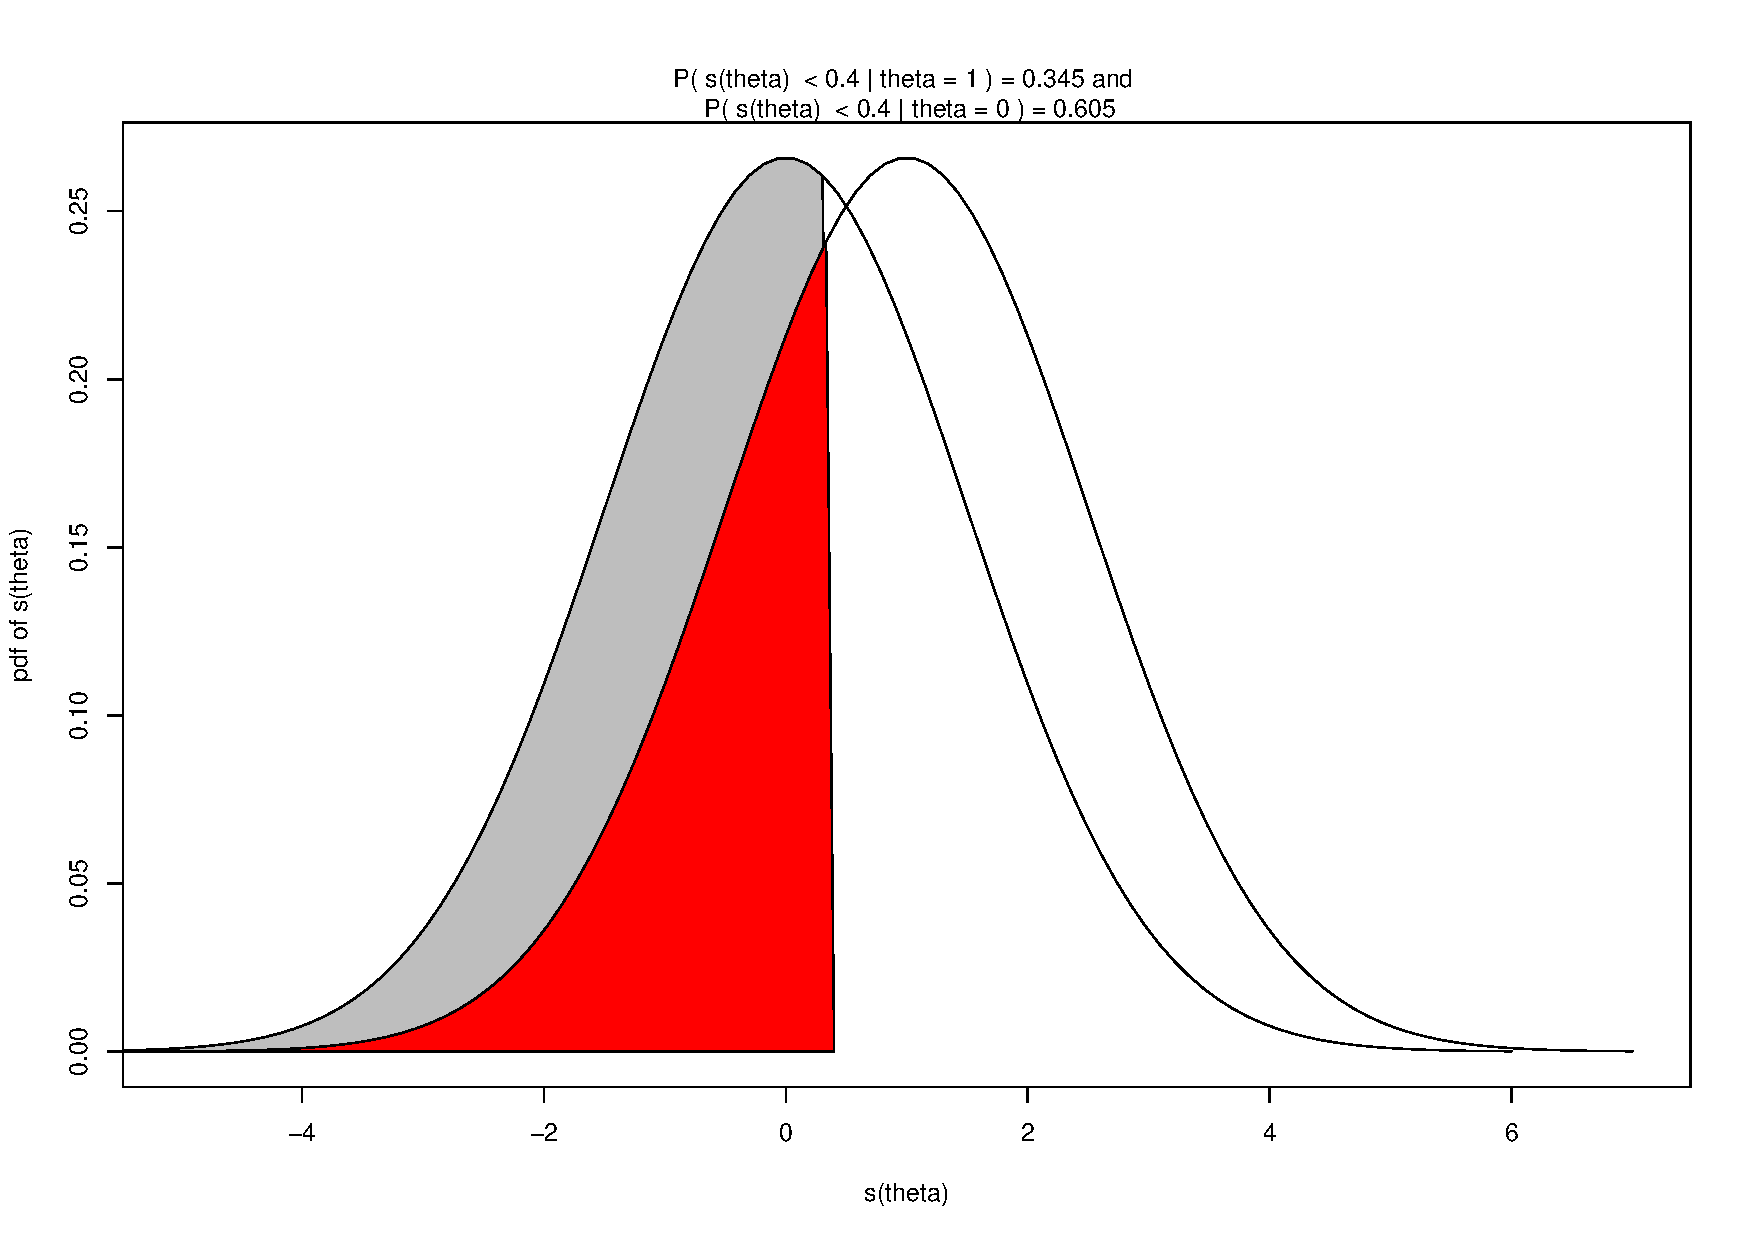
\includegraphics[width=\textwidth]{pdf_1.pdf}
\caption{$\pi(s \leq 0.4 | \theta = 0, \hat{\sigma}^2 =  2.25)$ in grey and $\pi(s \leq 0.4 | \theta = 1, \hat{\sigma}^2 =  2.25)$ in red}
\label{fig:pdf_1}
\end{figure}

\noindent Now, a critical assumption of the model is that \textit{only} $S$ is fully informed about $R$'s objective function and his prior beliefs. $R$ only knows for certain that $S$ cannot send any biased information and therefore holds an exogenous belief about her signal's distribution: $s(\theta)\sim(\theta, \hat{\sigma}^2)$ . Thus, by assumption, $\hat{\sigma}^2$ is not endogenous to the level of transparency $\sigma^{*2}_{H,L}$ that $S$ chooses in equilibrium. An admittedly strong restriction, which should however avoid a form of Lucas critique of rational expectations: If $R$ were fully informed, he could anticipate $S$'s level of transparency under both potential states of the world (though he still does not know which of them is true) and adjust his belief such that he could now weight received signals congruent with their actual probability distribution, which changes his posterior distribution for different values of $s$. As a consequence, the initial cut-off $s^{*}$ would change, inducing $S$ to choose a new $\sigma^{*2}_{H,L}$. A change that $R$ would again anticipate, adjust his belief and so on. No equilibrium in pure strategies could be found in that case, because $R$ could not credibly commit to a certain belief $\hat{\sigma}^2$ and every adjustment of $\hat{\sigma}^2$ would induce a new $\sigma^{*2}_{H,L}$. But failure to find a pure strategy equilibrium is not a sufficient argument to make such a restrictive assumption. In fact, I argue that the exogeneity assumption of $R$'s belief about $S$'s transparency is necessary in order to accurately map the real-life situations in which this sort of communication occurs. Let's consider the example of the FOMC providing information about the state of the economy to US Congress: The Congressmen know that the FOMC cannot bias its minutes, as the lies would be revealed 5 years later when the FOMC transcripts become open for access\footnote{Due to the US Transcript Act from 1993}, which would as a consequence severely damage the Fed's credibility and reputation.\footnote{We can further find substantive empirical evidence in the literature and in \citet{GL2017}, which shows that the communication between the Fed and the legislature is not a cheap talk game and contains no bias.} But just as much as the true state of the economy is exclusivly known to the FOMC, the cost of transparency from sharing this information remains private to the committee. It can be seen as additional expert knowledge, where only the FOMC knows how much explaining effort it requires to reveal more about the state of the economy. Or only the FOMC can predict how large negative externalities on the financial markets would be if it chose more transparency. Furthermore, a politician's belief about an expert's transparency can always experience exogenous shifts through negative media reports. For example, dismissive reports on the trustworthiness of experts in general or on the same sort of experts abroad can induce high $\hat{\sigma}^2$, independent of the actual level of an expert's transparency (i.e. $\sigma^2$). \citet{GL2017}'s work in progress tries to provide empirical evidence on such media-induced shifts in the public's belief of how transparent the FOMC communicates. Together with his already generated data, it should be possible to show how those shifts influence the actual level of transparency in communication between the US Congress and the FOMC. 

\noindent However, we have to consider what would happen if $R$ had the belief $\hat{\sigma}^2 = 0$ such that upon receiving a signal $s'=1$ he would update his prior to the following posterior:

\begin{center}
$\pi(\theta = 0|s',\hat{\sigma}^2=0)$ 
\end{center}

\begin{center}
$= \dfrac{\pi(s' | \theta = 0,\hat{\sigma}^2=0)\pi(\theta = 0)}{\pi(s' | \theta = 0,\hat{\sigma}^2=0)\pi(\theta = 0) + \pi(s'| \theta = 1,\hat{\sigma}^2=0)\pi(\theta = 1)}$
\end{center}

\begin{center}
$=\dfrac{(0)\pi(\theta = 0)}{(0)\pi(\theta = 0)+(1)\pi(\theta = 1)} = 0 < 0.5 \Rightarrow a_{R}=1$
\end{center}

\noindent As we can see, even if he had a strong prior $\pi(\theta = 0)>0.5$, the signal fully dominates his posterior due to his belief $\hat{\sigma}^2 = 0$ with which he assumes perfect signal precision and hence $\pi(s' | \theta = 0,\hat{\sigma}^2=0)=0$. In fact, this is true for all $\hat{\sigma}^2$ that would result in a fully revealing signal distribution: $R$ assumes that whatever signal he receives, he will be able to perfectly derive the true state from the world from it, placing all weight on the signal in his posterior. But the case $\hat{\sigma}^2 = 0$ most obviously shows what would happen if - as we know is true in equilibrium - $S$ then chooses a not perfectly revealing distribution that generates signals outside of 1 or 0, e.g. $s'=0.8$. Then $R$ would immediately learn that $\hat{\sigma}^2=0$ cannot be true. I therefore assume that $R$ always believes $s(\theta)\sim(\theta=0, \hat{\sigma}^2)$ and $s(\theta)\sim(\theta=1, \hat{\sigma}^2)$ to intersect, i.e. he knows that signal distributions are not fully revealing and hence always holds a belief $\hat{\sigma}^2 > (0.5/3)^2 \approx 0.028$. Ultimately, we have a set-up in which it is common knowledge that $S$ does never choose a level of transparency $\sigma^2 \leq 0.028$.

\subsection{Introducing Receiver Types:}

\noindent Given the equilibrium for $\sigma^{*2}_{H,L}$ that I found, I am now going to introduce two types of receivers: A congruent ($c$) and a non-congruent ($nc$) type with priors $\pi_{c}(\theta=0) < 0.5 < \pi_{nc}(\theta=0)$, i.e. the congruent type's prior belief that the state of the world is high is higher than the non-congruent's. So the non-congruent type needs a more convincing signal when $\theta=1$ in order to make him choose a high action $a_R =1$. The terms congruent and non-congruent type are borrowed from Dewatripont and Tirole (2005), where the authors use them to derive different equilibrium levels of effort for both receiver and sender in order to successfully communicate with each other. Again, the difference here is that the sender $S$ cannot choose zero cost (which would be zero effort in Dewatripont and Tirole (2005)) without risking a false choice of action by the receiver $R$, even if $R$'s prior is biased towards the true state of the world. Empirically, a congruent type could represent a Democrat Congressman  whose prior belief tends towards taking high policy action, such as increasing government expenditure or other interventionist market policies. On the other hand, a non-congruent type could represent a Republican Congressman whose prior belief leans towards low policy action, such as non-intervention in markets, low government expenditure and low taxation. Hence, if the state of the world asks for high action $a_{R}=1$, it would be harder for an expert committee such as the FOMC to persuade a Republican Congressman. A signal sent to a Republican would therefore need to be stronger than one sent to a Democrat, which means that the action cut-off value $s^{*}$ is higher for the Republican (i.e. closer to 1 than to 0), independent of his belief $\hat{\sigma}^2$. Vice versa, if the state of the world demands a low action, the Democrat would need more persuasion, as his threshold $s^{*}$ lies lower (i.e. closer to 0 than to 1), independent of his belief $\hat{\sigma}^2$. 

\subsection{Comparative Statics}

\noindent In this section I first explain the comparative statics results we can derive from the model. In the second part, I show how these apply to empirical evidence from \citet{GL2017}, which shows that transparency in communication between the FOMC and US Congress increases when the state of the economy is bad (requiring high action $a_{R}=1$).

\subsection{Summary of Results:}

\noindent We can derive the following results from the above presented model and its PBE in pure strategies:

\begin{enumerate}
\item $\sigma^{*2}_H$ (i.e. when $\theta = 1$) is lower for non-congruent types with low priors (i.e. $\pi_{nc}(\theta = 0)>0.5$). $\sigma^{*2}_L$ (i.e. when $\theta = 0$) is higher for non-congruent types. This means that $S$ sends a more precise signal to a non-congruent $R$ when the state of the world is high and a less precise signal when it is low.
\item $\sigma^{*2}_H$ (i.e. when $\theta = 1$) is higher for congruent types with high priors (i.e. $\pi_{nc}(\theta = 0)<0.5$). $\sigma^{*2}_L$ (i.e. when $\theta = 0$) is lower for congruent types. This means that $S$ sends a less precise signal to a congruent $R$ when the state of the world is high and a more precise signal when it is low.
\item $\sigma^{*2}_H$ and $\sigma^{*2}_L$ additionally depend on $\hat{\sigma}^2$. For a non-congruent type, $\sigma^{*2}_H$ is even lower the more untrusting $R$ is (i.e. he has a high $\hat{\sigma}^2$).\footnote{As long as $\hat{\sigma}^2 < +\infty$, because we know that we otherwise have a babbling equilibrium with no transparency at all: $\sigma^{*2}_{H,L} \to +\infty$.} Trivially, $\sigma^{*2}_H$ is higher if he is more trusting and has low $\hat{\sigma}^2$. A high $\hat{\sigma}^2$ means that $R$ weighs the signal less in his posterior.\footnote{$\pi(s' \leq s | \theta = 0,\hat{\sigma}^2=0)$ decreases relative to $\pi(\theta = 0)$ as $\hat{\sigma}^2$ increases, where $s'$ is the signal received.} Hence, as $\hat{\sigma}^2$ increases, the action cut-off value $s^{*}$ moves closer to zero for a non-congruent types, which induces $S$ to choose a higher precision level such that all signals in the distribution are relatively high.
\item For a congruent type, $\sigma^{*2}_L$ is even lower the more untrusting $R$ is (i.e. he has a high $\hat{\sigma}^2$). Again trivially, $\sigma^{*2}_L$ is higher if he is more trusting and has low $\hat{\sigma}^2$. As $\hat{\sigma}^2$ increases, the action cut-off value $s^{*}$ moves closer to 1 for congruent types, which induces $S$ to choose a higher precision level such that all signals in the distribution are relatively low. This resembles an accountability effect, as negative exogenous shocks to $\hat{\sigma}^2$ cause \textit{more} transparent signalling. $S$ is held "accountable" for losing some of $R$'s trust by having to choose higher precision in her signal, which is costly (and hence a punishment)
\item A high transparency cost $c(\sigma^2)$ is always bad for both $S$ and $R$, such that their expected equilibrium utilities decrease in the constant $b$, which determines the baseline cost of transparency $e^{(b)}$. Because we know that the cut-off $s^{*}$ is endogenous to both $\hat{\sigma}^2$ and $R$'s prior $\pi(\theta = 0)$, we can state it as a function of both parameters $s^{*} = s^{*}(\hat{\sigma}^2,\pi(\theta = 0))$, where the expected equilibrium utilities are:
\end{enumerate}
\begin{equation*} 
EU_S=[-P(s \leq s^{*}|\hat{\sigma}^2,\theta=1)-c(\sigma^{*2}_{H})]\pi(\theta = 1)+[-P(s^{*} < s|\hat{\sigma}^2,\theta=0)-c(\sigma^{*2}_{L})]\pi(\theta = 0) 
\end{equation*}
\begin{center}
and
\end{center}
\begin{equation*}
EU_R=-P(s \leq s^{*}|\hat{\sigma}^2,\theta=1)\pi(\theta = 1) - P(s^{*} < s|\hat{\sigma}^2,\theta=0)\pi(\theta = 0)
\end{equation*}

\noindent These results allow for even more extended insights: Consider a group of receivers $R$ instead of only one and the group has to decide about action $a_R$ by unanimity rule. We can see that it is sufficient to have one non-congruent type among otherwise all congruent types in order to make $S$ choose the more precise signal distribution $\sigma^{*2}_H$ to persuade the non-congruent type when the state of the world is low. If they were all congruent, $S$ would choose a lower $\sigma^{*2}_H$ in equilibrium, as everyone's cut-off $s^{*}$ would be low. Hence, everyone else in the group benefits from higher transparency induced by the non-congruent type. Furthermore, if the non-congruent type among the congruent ones in the group is of the untrusting kind, then $S$ chooses an even higher precision level for the signal when $\theta = 1$. Can we derive a negative effect of having a non-congruent, untrusting type in the group when the state of the world is instead low? No, because then $S$ still chooses the higher precision level $\sigma^{*2}_L$ to persuade the congruent types in the group. And again, if they are also of the untrusting kind, transparency in the signal will be even higher. Obviously, the same positive spillover effect works when there are one or more congruent types in a group of otherwise non-congruent types. Hence, whenever we have a mix of high and low priors in a group, everyone benefits from the higher precision levels in the signal distribution under both states of the world. Now, a more interesting decision-making rule to consider is majority rule. If we now again have a group of congruent types and one non-congruent, the positive spillover from before no longer exists. $S$ only needs to persuade a majority in the group to take the high action when $\theta = 1$ such that the non-congruent's posterior becomes irrelevant under majority rule. When the state of the world is low, $S$ chooses the higher precision level $\sigma^{*2}_L$ in order to persuade the majority of congruent types (from which the non-congruent type benefits). Hence, with majority rule $\sigma^{*2}_{H,L}$ depends on the majority's prior beliefs, while with unanimity rule it depends on the type(s) in the group that are the most difficult to persuade. 

\subsection{Empirical Evidence on the Communication between FOMC and US Congress:}

\noindent \citet{GL2017} shows in his paper \textit{"Political Determinants of FOMC Transparency"} that overlapping wording between FOMC minutes and transcripts increases when economic news are bad, and even more so when at the same time a Congressional hearing of the Fed's chair comes up.\footnote{He controls for the length of the minutes and transcripts and the results are robust to it.} He uses 144 minutes and transcripts from the sample period 1993-2010. FOMC minutes are published and publicly accessible always 3 weeks after an FOMC meeting and are not only informative to politicians but also to the financial markets. They summarize the meeting's discussion between the members of the committee as well as their decision outcomes on monetary policy. The FOMC transcripts, on the other hand, are publsihed only 5 years after a meeting and are an accurate script of all statements made during the meeting. Hence, we can find out everything that was said in a meeting once we read the transcript, while we only receive partial information on that in the minutes. The FOMC can decide how much to reveal in the minutes, but if they would lie about certain information, it would become public 5 years later with the publication of the transcripts. \citet{GL2017} argues that this observed sensitivity in transparency (i.e. the overlapping of the wording between minutes and transcripts) resembles an accountability effect, where the Fed feels obliged to report more openly to Congress when economic news are bad, which might be related to the Fed's policies.\footnote{Before coming to that conclusion, he further needs to provide evidence that the rate of overlapping words does not simply increase due to more complex language during bad economic times, which would make the use of simpler or summarising language in the FOMC minutes more difficult than when the economy goes well.} My model offers an alternative interpretation of Lisi's results and further suggests an extension to the empirical research design. If we consider the US Congress as a group of receivers $R$ and the FOMC as a single sender $S$, we could interpret Republican Congressmen as non-congruent types, which need more persuasion to choose a high action $a_R$. Actions are in this case policies and high action is required when the state of the economy is bad (i.e. $\theta = 1$). The worse the economy the more would the FOMC need Congress to support its monetary policy of low interest rates (and potentially also quantitative easing) with government expenditure or other interventionist measures that do not counteract but instead support the Fed's intention to revive the economy. In the US, Congress has decision-making power over the government budget and is therefore the one that needs to be persuaded for high action. Democrat Congressmen represent congruent types, which need less persuasion for high action when the economy is bad, but more persuasion for low action when the economy booms. Again, this has an empirical intuition: When the economy is booming (i.e. economic news are good), the FOMC needs Congress to support its anti-inflationary policy of high interest rates by curbing government expenditure, which represents low action $a_{R}=0$. Democrats usually need more persuasion than Republicans to do so. Hence, they have a lower cut-off $s^{*}$ and therefore need a lower signal in order to persuade them to take low action than Republicans do, implying that Republicans have a high cut-off $s^{*}$. Now, if both Senate and House have a Republican majority such as during the late Clinton and early Bush terms (see figure~\ref{fig:congress}), the FOMC should have been more transparent during bad than during good economic times. And vice versa, when both Senate and House had a Democrat majority such as during the early Clinton and Obama terms, the FOMC should have been more transparent during good than during bad economic times. But the model shows that for always higher transparency, Senate and House need to be split between the Republican party ruling one and the Democrat party ruling the other. Just like with unanimity rule, a mix of a non-congruent majority in e.g. the House and a congruent majority in e.g. the Senate induces the FOMC to always send more precise signals about the state of the economy (and implicitly the required action), as in good times the Senate would need stronger persuasion and in bad times the House. Both House and Senate have to agree to a policy bill such that the two chambers have to make a unanimous decision. \citet{GL2017} does not make a distinction between Republican and Democrat majorities in either Senate or House in his OLS regression (see Appendix). However, my model suggests that he should control for a Republican majority in either House or Senate during the sample period such that he would need to run the following regression:
\begin{equation*}
Transparency_{t,q}= \alpha + \gamma_{t} + \sigma_{q} + \beta_{1}News_{t,q} + \beta_{2}Rep_{t,q} + \beta_{3}(News*Rep)_{t,q} + \epsilon_{t,q}
\end{equation*}
\noindent where the dependent variable is his earlier described indicator for transparency in FOMC's communication in quarter $q$ in year $t$. $\gamma_{t}$ is controlling for year effects and $\sigma_{q}$ for quarter effects (i.e. for quarters 1 to 4). The independent variable are his continuous measure for bad economic news $News_{t,q}$ where higher values indicate worse news. Finally, the newly introduced binary variable $Rep_{t,q}$ for a Republican majority in either House or Senate should be complemented by the interaction variable $(News*Rep)_{t,q}$, which captures the effect of interest: As economic news go bad, is FOMC transparency significantly higher when Republicans rule either House or Senate or both? The problem he will however face empirically is that his sample of 144 observations does not provide sufficient power to introduce these additional two controls. He therefore needs to extend his sample to years before 1993, which is work in progress.\footnote{The US Federal Reserve exists since 1913.} With an extended sample, he could further test for a positive, significant year-news interaction effect on FOMC transparency based on the following hypothesis: Empirical observation in more recent years have led to a large group of scholars claiming that the Republican party has become more extreme and hence the US party landscape has polarized. If that is also true for the economic policy dimension, then the Republican prior $\pi(\theta=0)$ must have shifted towards 1, implying that it is nowadays harder to persuade Republicans that the state of the economy requires high action (i.e. government spending). Thus, necessary precision in the signal's distribution needed to be higher when the economy was doing badly in recent years, which should have induced a stronger positive effect of bad news on FOMC transparency. Especially, as there was only one period between 2008 and 2012, where both House and Senate were ruled by the Democrats (see figure~\ref{fig:congress}).

\begin{figure}[h]
\centering
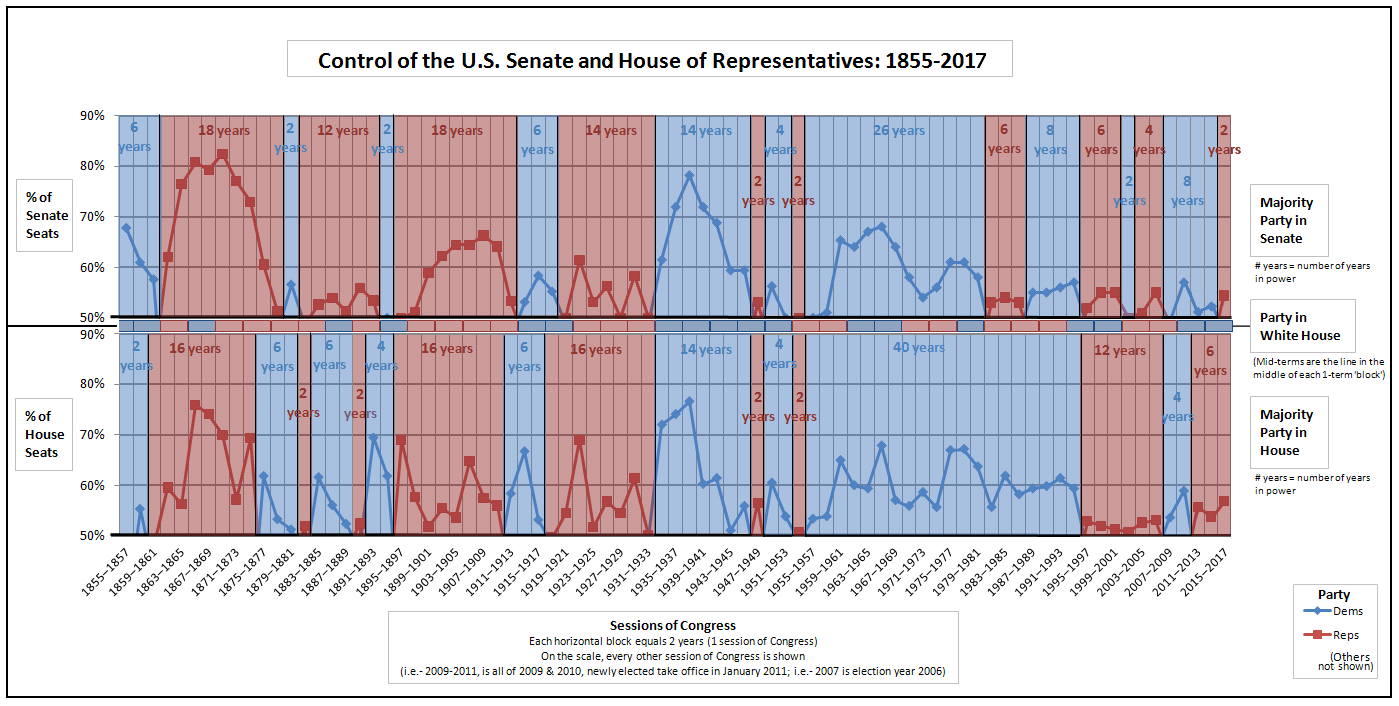
\includegraphics[width=\textwidth]{congress.png}
\caption{Majority Control in the US Senate and House of Representatives, 1855-2017. \textit{Source:} Wikipedia (2017), Uspolitics.about (2017), Filibustercartoons (2017) and Infoplease (2017).}
\label{fig:congress}
\end{figure}

%Wikipedia (2017), Uspolitics.about (2017), Filibustercartoons (2017) and Infoplease (2017)

\noindent To recall, Lisi's current results show a significant positive effect of bad news on FOMC transparency and a significant positive interaction effect between bad news and upcoming Congressional hearings (see Appendix). But this paper's model suggests that what his effect may capture is that Republicans simply have stronger priors. Hence, their cut-offs $s^{*}$ have a more narrow proximity to 0 than Democrats' cut-offs have to 1. This therefore induces more precise signalling in bad economic times when the Republican, non-congruent type has to be persuaded than in good economic times when the congruent Democrats need persuasion. The fact that the sample 1993-2010 contains more years with at least one of the two chambers being ruled by the Republican party supports this hypothesis. The positive effect of bad news (and hence the need for Republican persuasion) should be even stronger when Republicans are mistrusting the FOMC (i.e. if they think FOMC communication is not very transparent). As a consequence, \citet{GL2017} would be right that there is indeed some kinf of accountability effect at work, just not the one he suggested. According to my model, the FOMC is not more transparent as a reaction to bad economic news, but instead as a reaction to less trusting Republican majorities in Congress. Lisi's work in progress uses media data that accounts for bad news on central banks and monetary policy, which could allow for an empirical test whether media-induced shifts in Congressmen's beliefs about the FOMC's transparency (i.e. $\hat{\sigma}^2$) boosts its actual transparency (i.e. $\sigma^2$). However, those shocks should be exogenous in order to allow for a valid test of this hypothesis.\footnote{He could for example test the effect of negative news about foreign central banks or, as suggested earlier in the paper, (foreign) news about the trustworthiness of experts in general.} Further evidence from \citet{GL2017} shows a significant negative effect of Congressional hearings on FOMC transparency when economic news are good. Thus, the FOMC significantly lowers transparency when a Congressional hearing is coming up while the economy is doing well. An admittedly speculative but still possible explanation could be that upcoming Congressional hearings coincide with lower $\hat{\sigma}^2$, which means that Congress assumes that the FOMC is more transparent when a hearing comes up. Hearings were introduced to improve communication between US Congress and FOMC such that Congress could indeed expect a positive accountability effect on FOMC transparency when a hearing comes up. But according to my model, that expectation would exactly cause less precision in the FOMC's signalling than if expectations about $\hat{\sigma}^2$ were high. However, this cannot be true. Because when economic news are bad, Lisi's results show that an upcoming Congressional hearing has a significant positive effect on the committee's transparency, while without the hearing coming up, the effect of bad news is insignificant. It would therefore need to be that only Democrats assume that hearings cause a lower $\hat{\sigma}^2$ and Republicans actually hold an opposite belief. Alternatively, it could be that shifts in $\hat{\sigma}^2$ before an upcoming hearing interact with the state of the economy: During good economic times, Congressmen believe that the FOMC will report more openly when a hearing is imminent, while during bad times Congress thinks that the FOMC tries to hide more before a hearing. However, these hypotheses are built on less solid ground and would need at least supportive anecdotal evidence to be worth testing. Important to know is that the timing of Congressional hearings is always exogenous, as it follows an across years fixed schedule. Upcoming hearings therefore do not depend on the state of the economy. 

\noindent At last, it seems important to ensure that the model's assumptions fit with the empirical example of the FOMC's communication with US Congress. First, their objective functions make sense: The FOMC as sender cares about Congress receiving the right signal such that economic policy matches the state of the world and the FOMC's monetary policy. The Congress's and the Fed's policy should never counteract. The FOMC does further indeed have access to exclusive knowledge about the state of the economy, which it passes on to Congress (and in fact the public) in his published minutes. Monetary policy itself is always an indicator of the state of the world, but its scope is limited and Congress is therefore still depending on what exactly the FOMC communicates about the state of the economy (and hence the required action). Thus, Congress also wants to choose the right policy that perfectly matches the state of world, but it has (party-dependent) priors about the likelihood of each state. Important is that the FOMC indeed faces a probably exponential cost to transparency. Out of the two given reasons why transparency can be costly, the second seems to apply more urgently to the FOMC. Whatever message the FOMC sends to Congress about the state of the economy, it has potential negative externalities on the financial markets. As the FOMC minutes are publicly accessible and widely read by banks and traders, too precise information can cause damaging behavioural reactions such as a credit crunch when the state of the economy is bad or speculative trading when it is good. Too much transparency in the FOMC minutes therefore risks that financial markets counteract to the Fed's policy (e.g. in the case of banks freezing their credit issuance while the Fed tries to revive the economy with low interest rates). Even worse, too much transparency would at the same time also counteract to Congress's policy (e.g. a credit crunch would make higher government expenditure ineffective). Second, I have already shown that congruent and non-congruent type distinction fits especially well in the case of the US Congress. Third,   it is most likely true that Congress never assumes the FOMC to communicate fully revealing, which appears fair just by the sheer fact that the published FOMC minutes are always a summary of the held meetings and can hence \textit{never} contain everyhting said and discussed. But at the same time, it seems valid to assume that Congress holds an exogenous belief about the FOMC's transparency. Earlier in the paper I gave detailed reasons for why that is. 

\subsection{Welfare Effects:}

\noindent The model shown in this paper has a number of social welfare implications if we assume that more transparent communication between experts and legislators or the public is welfare-enhancing. The implications result directly from the comparative statics analysis made in this section:

\begin{enumerate}
\item Under unanimous decision-making, it is welfare-enhancing to have variation in priors among the receivers. In equilibrium the sender chooses a precision level to persuade the one(s) with the most extreme prior. It is therefore welfare-ehancing to have the rule of the two chambers in US Congress split between the Democrat and the Republican party. 
\item The more extreme the priors $\pi(\theta = 0)$ the receivers have, the more precise is the signal the sender sends. From a transparency point of view, political polarization in the US is therefore welfare-enhancing, as it implies receivers with a very high or a very low prior $\pi(\theta = 0)$. In order to boost transparency, the receivers however cannot have too strong priors, because they still need to place some weight onto the signal they receive.
\item Transparency is even higher when the receivers that are hard to persuade do not trust the sender (i.e. they have high $\hat{\sigma}^2$ beliefs). Hence, in the case where Congress chambers are split between a Democrat majority in one and a Republican majority in the other, mistrusting experts pays off, independent of the state of the world. This resembles an accountability effect, as experts like the FOMC increase their transparency in communication as a response to mistrust of receivers that are already hard to persuade.
\item Third-party externalities: When the signal is not entirely exclusive to the receiver who shares the same objective as the sender, then signal precision is costly and hence constrained. The earlier given example are financial markets reacting to what state of the economy the FOMC communicates to US Congress. From this follows a potential policy implication: Should the Federal Reserve and Congress be able to communicate through an exclusive channel? Given their objective functions, if exclusive communication could fully eliminate the cost of transparency for the FOMC, it would always fully inform the Congress about the state of the economy. As a consequence, both Fed and Congress could always choose complementary or even synergetic economic policies that do not counteract. Resulting welfare effects could be significant. However, exclusive communication between the Fed and Congress could obviously put the Fed's independence at risk - a trade-off that only few among us would be willing to make.
\end{enumerate}

\section{Conclusion}

In this paper I provide a formal model of situations in which open communication between two independent agents that pursue the same objective is constrained by an exponential cost of transparency for the message sender. The receiver(s) hold(s) a prior belief about the state of the world, based on which he wants to choose the right action, and on the level of transparency with which the sender communicates. Upon receiving the signal from the sender, the receiver forms a posterior on the state of the world using Bayesian updating. His prior belief about the sender's transparency is however exogenous. I show that if the baseline cost is not too high, we can always find an informative equilibrium in pure strategies in which the sender chooses an unbiased signal distribution at an optimal level of transparency (i.e. the distribution variance), which is when the marginal increase in the expected loss matches the marginal decrease in cost from less transparency. A babbling equilibrium with no valuable information exchange occurs more often as the baseline cost grows and whenever the receiver(s) believe that the sender is completely intransparent. Equilibrium transparency levels improve with the level of persuasion that is needed to convince the sender about true state of the world. We learn that equilibrium transparency is even higher when in addition the receivers also find the sender not very trustworthy (i.e. when their prior beliefs about the variance in his signal increase). These findings have interesting welfare implications, which suggest that it can often pay off to mistrust experts. Further, to have a mixed group of receivers is beneficial, as different priors allow for positive spillover effects. The sender always addresses the receivers in the group that are the hardest to persuade such that the others also benefit from the lower variance in the signal distribution. Using majority instead of unanimity rule to decide about what action to take weakens this positive spillover effect, as now the sender no longer has to persuade all receivers in the group. At last, when transparency is costly due to negative externalities that the non-exclusivity of the signal induces, then it can be welfare-enhancing to allow for an exclusive communication channel between sender and receiver. Empirical evidence on the communication between the US federal open market committee and the US Congress by \citet{GL2017} complements this paper's model. The evidence we find indicates that a Republican majority in either House or Senate induces more transparency in the FOMC's communication when the state of the economy is bad and requires interventionist policy action such as more government spending. Less obvious are empirical results showing that an upcoming Congressional hearing positively interacts with bad, but negatively interacts with good news. One possibility in accordance with the model would be that Congress's belief about the FOMC's transparency increases when a hearing comes up in good and decreases in advance to a hearing in bad times. Any sort of positive reaction in FOMC transparency to an increase in Congress's mistrust resembles an accountability effect.

For further empirical contributions to this paper, \citet{GL2017} should extend his sample of FOMC meetings to years before 1993 and introduce a control for a Republican majority in either House or Senate per year and and measure its interaction with bad news. Also, he should test for a year-news effect, which could capture a likely shift in the Republican prior over the past years, which should have had a positive effect on FOMC transparency. Further, he should analyse his current work-in-progress media data on negative shocks to the FOMC's reputation, which should induce higher transparency as a response to more mistrust by Congress. An analysis of the Congressional hearings transcripts could provide information on the prior beliefs that the party majorities of the two Congressional chambers hold about the state of the economy (and implicitly the required policy action) and the transparency of the FOMC. It is also essential that the used indicator for transparency is valid. \citet{GL2017} should therefore provide evidence that eliminates the concern that higher similarity between FOMC minutes and transcripts in economically bad times simply reflects the more complex or technical language used in those periods. To test whether exclusive communication channels allow more open communication, we could analyse the information exchange between experts and politicians such as in US presidential meetings when transcripts become public a few years later.

\section{Appendix}

\subsection{Proof I:}

I. $\theta=1$:
\begin{equation}
\dfrac{\partial P(s \leq s^{*}|\hat{\sigma}^2,\theta=1)}{\partial \sigma^{2}} = \dfrac{\partial F(s^{*})}{\partial \sigma^2} = \dfrac{\partial \Phi(\dfrac{s^{*}-\theta}{\sqrt{\sigma^2}})}{\partial \sigma^2} = \phi\Big(\dfrac{s^{*}-\theta}{\sqrt{\sigma^2}}\Big)\Big(\dfrac{s^{*}-\theta}{2\sigma^{\frac{3}{2}}}\Big) < 0
\end{equation}

where $s^{*}>\theta$ and hence $\phi\Big(\dfrac{s^{*}-\theta}{\sqrt{\sigma^2}}\Big)<0$ and $\Big(\dfrac{s^{*}-\theta}{2\sigma^{\frac{3}{2}}}\Big)>0$

II. $\theta=0$:
\begin{equation}
\dfrac{\partial P(s^{*} < s|\hat{\sigma}^2,\theta=0)}{\partial \sigma^{2}} = \dfrac{\partial (1-F(s^{*}))}{\partial \sigma^2} = \dfrac{\partial (1-\Phi(\dfrac{s^{*}-\theta}{\sqrt{\sigma^2}}))}{\partial \sigma^2} = \phi\Big(\dfrac{s^{*}-\theta}{\sqrt{\sigma^2}}\Big)\Big(\dfrac{s^{*}-\theta}{2\sigma^{\frac{3}{2}}}\Big) > 0
\end{equation}

where $s^{*}<\theta$ and hence $\phi\Big(\dfrac{s^{*}-\theta}{\sqrt{\sigma^2}}\Big)<0$ and $\Big(\dfrac{s^{*}-\theta}{2\sigma^{\frac{3}{2}}}\Big)<0$

\subsection{Proof II:}

Value of cut-off signal $s^{*}$:

$s^{*}$ is such that 

\begin{center}
$\pi(\theta = 0|s^{*},\hat{\sigma}^2)$ 
\end{center}

\begin{center}
$= \dfrac{\pi(s^{*} | \theta = 0,\hat{\sigma}^2)\pi(\theta = 0)}{\pi(s^{*} | \theta = 0,\hat{\sigma}^2)\pi(\theta = 0) + \pi(s^{*} | \theta = 1,\hat{\sigma}^2)\pi(\theta = 1)} = 0.5$
\end{center}

\begin{center}
$\iff \pi(s^{*}|\theta = 0,\hat{\sigma}^2) = 1 - \pi(\theta = 0) = \pi(\theta = 1)=\pi(s^{*}|\theta = 1,\hat{\sigma}^2)$ 
\end{center}

where the exact value of $s^{*}$ depends on the exact value of $\hat{\sigma}^2$ and $\pi(\theta = 0)$

\subsection{Proof III:} Proving that $S$ never chooses a fully revealing signal distribution.

Assume that $s(\theta)\sim(\theta, \sigma^{*2})$ was a fully revealing signal distribution, then increasing $\sigma^{2}$ should not be a profitable deviation.

From the first order condition in (3) we know that $S$ chooses $\sigma^{*2}$ such that:

\begin{equation}
\phi\Big(\dfrac{s^{*}-\theta}{\sqrt{\sigma^{*2}}}\Big)\Big(\dfrac{s^{*}-\theta}{2\sigma^{\frac{3}{2}}}\Big) = e^{(-\sigma^{*2} + b)}
\end{equation}

where this equality does not hold but instead

\begin{equation}
\phi\Big(\dfrac{s^{*}-\theta}{\sqrt{\sigma^{*2}}}\Big)\Big(\dfrac{s^{*}-\theta}{2\sigma^{\frac{3}{2}}}\Big) < e^{(-\sigma^{*2} + b)}
\end{equation}

as $\sigma^{*2} \approx \Big(\dfrac{s^{*}-\theta}{3}\Big)$ and hence $e^{(-\sigma^{*2} + b)}<1$. And $\phi\Big(\dfrac{s^{*}-\theta}{\sqrt{\sigma^{*2}}}\Big)\Big(\dfrac{s^{*}-\theta}{2\sigma^{\frac{3}{2}}}\Big)<1$ as $\phi\Big(\dfrac{s^{*}-\theta}{\sqrt{\sigma^{*2}}}\Big) \leq 1$ and $0<s^{*}<1$ such that $\Big(\dfrac{s^{*}-\theta}{2\sigma^{\frac{3}{2}}}\Big)<1$. 

Such that:

\begin{equation}
\dfrac{\phi\Big(\dfrac{s^{*}-\theta}{\sqrt{\sigma^{*2}}}\Big)\Big(\dfrac{s^{*}-\theta}{2\sigma^{\frac{3}{2}}}\Big)}{e^{(-\sigma^{*2} + b)}}<1
\end{equation}

and therefore $S$ would always have an incentive to deviate from a fully revealing signal distribution.


\subsection{OLS Output from \citep{GL2017}:}
\begin{figure}[h]
\centering
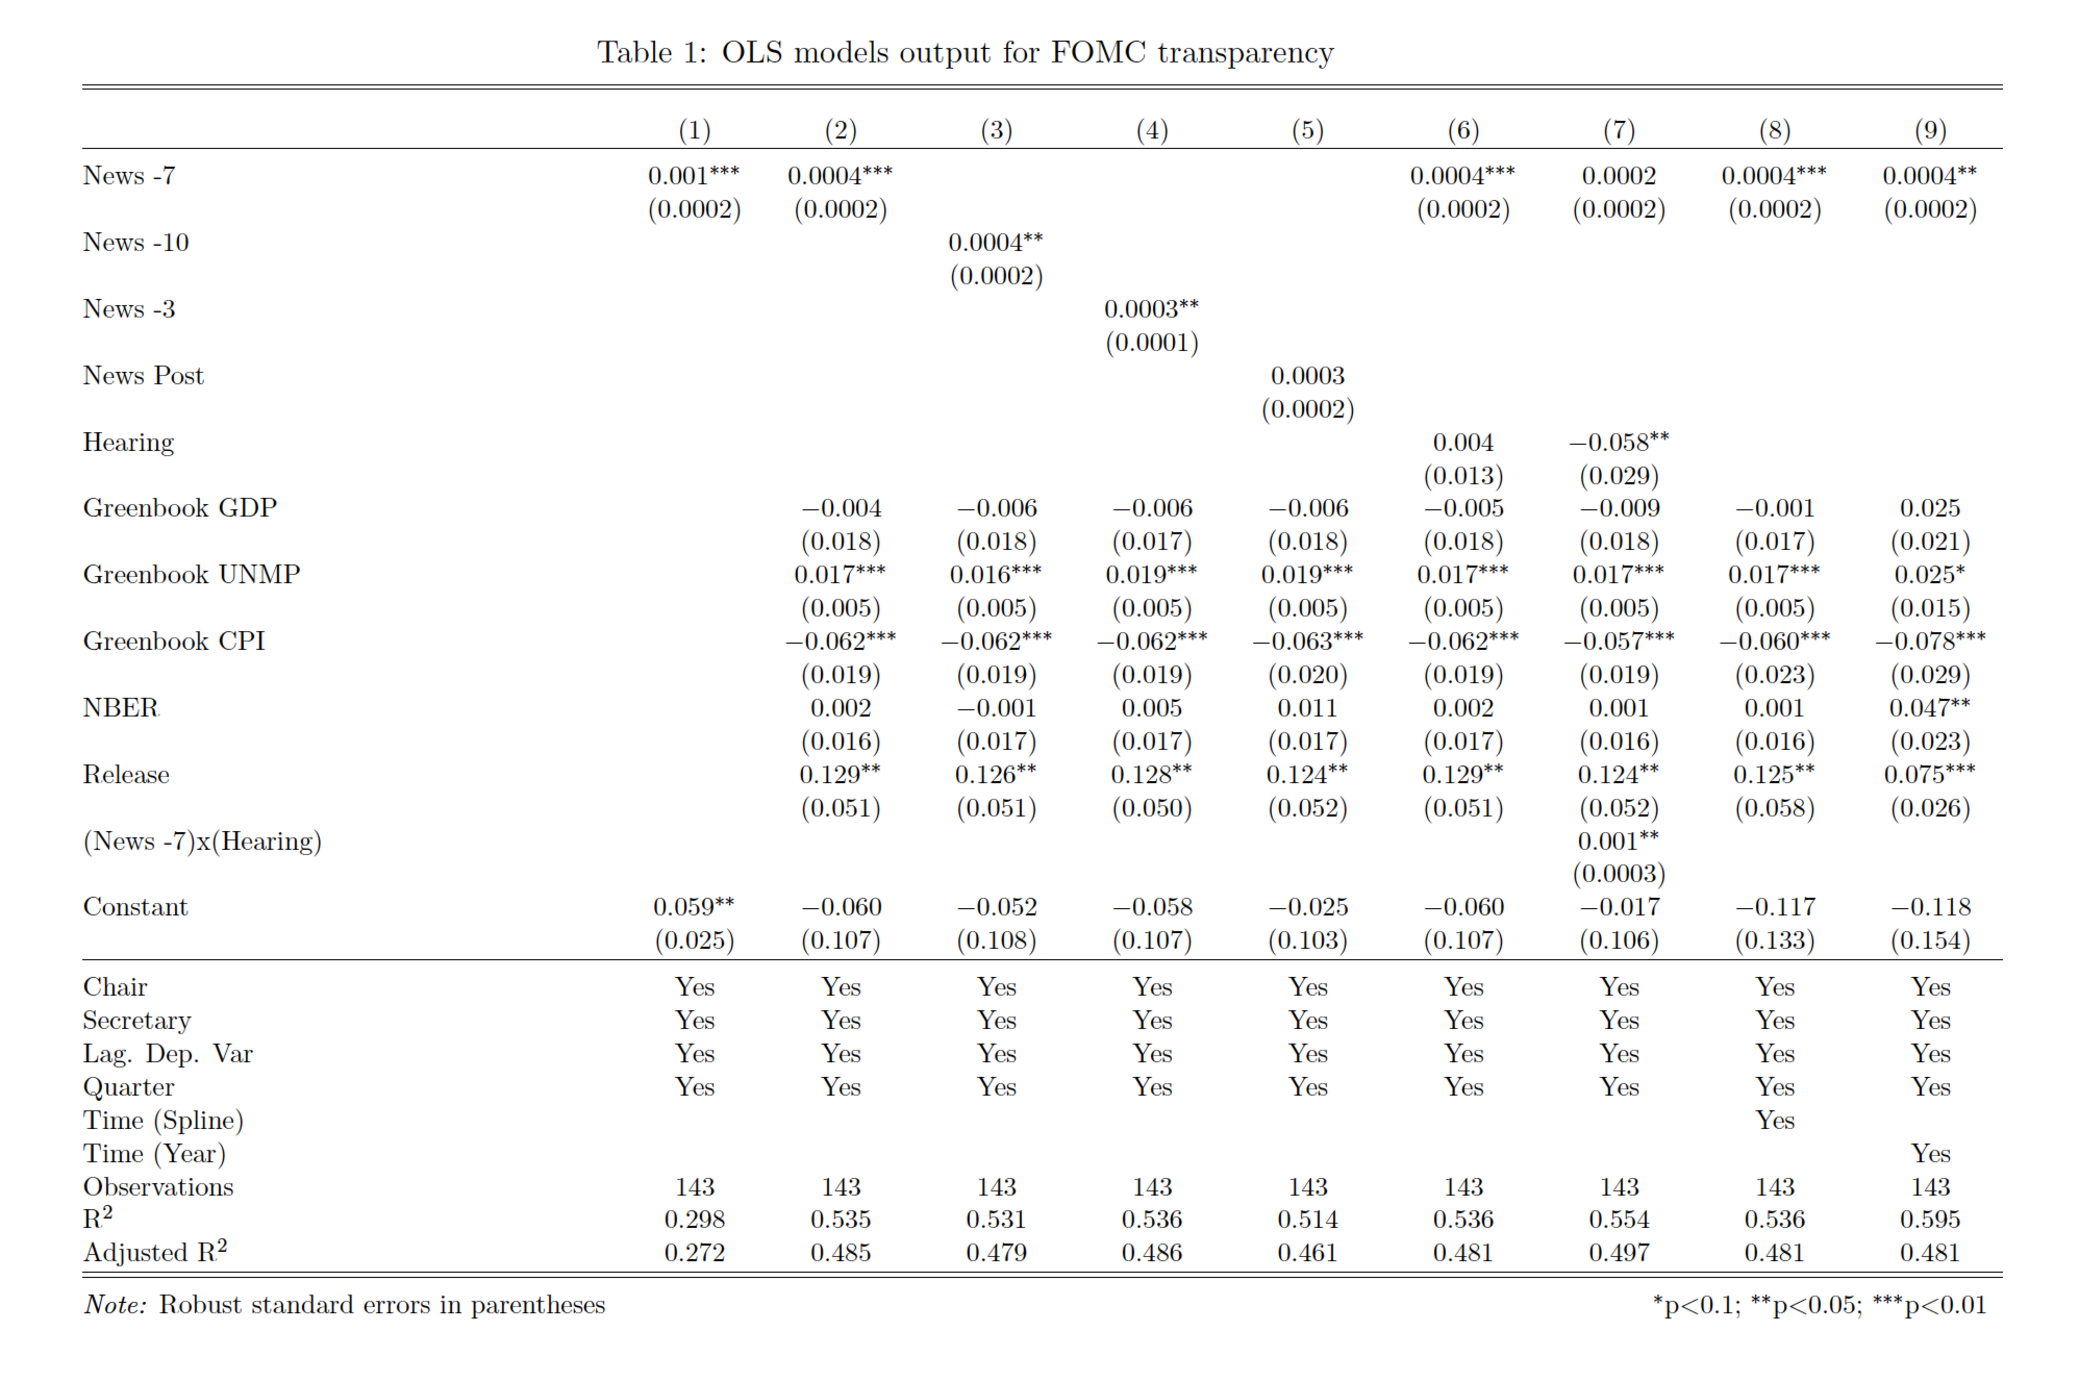
\includegraphics[width=\textwidth]{ols.pdf}
\caption{The effect of news (where larger numbers indicate worse news) on FOMC transparency (i.e. cosine similarity of text between 144 FOMC minutes and transcripts), 1993-2010 \citep{GL2017}.}
\label{fig:ols}
\end{figure}

% ============================================== %
% BIBLIOGRAPHY ============================ %
% ============================================== %

\newpage
\nocite{*}
\bibliographystyle{plainnat}
\bibliography{bureaucrat_persuasion_model_biblio}


\end{document}